\documentclass[a4paper,11pt]{article}
\usepackage[utf8]{inputenc}
\usepackage{hyperref}
\usepackage{graphicx}

%opening

\title{Cross-linguistic replication study on politeness}
\author{P. Tsvilodub, L. Schießer, C. Eckert, M. Zeller 
\\ \textit{Experimental Psychology Lab Class, University of Osnabrück, Germany}}

\begin{document}

\maketitle
\begin{abstract}
The goals of being polite and informative in conversation at the same time do not seem to be compatible if the speaker is seen as a perfectly  rational cooperative agent. Specifically, this means that the speaker's only goal would be to transfer as much information as possible in an efficient way. The trade-off between politeness and informativity has been studied in a previous rating experiment conducted by Yoon et al. \cite{yoon2016talking} in 2016. The authors hypothesize that polite utterances are rationally explained as a trade-off between the communicative goal of informativity and social utility. We now wanted to find out if there are cross-linguistic differences in politeness interpretation by translating the rating experiment from English into German.     
\end{abstract}
\section{Introduction}
This experiment represents a replication of a part of an experiment done by Yoon et al. \cite{yoon2016talking}. This study was concerned with politeness, a technique we use in everyday life conversations with different intentions. One example could be that your friend is terrible at cooking, but in order not to offend him you will say that the meal tasted good. The problem is that politeness violates principles of a cooperative speaker, i.e. being informative and efficient updating the listener \cite{grice1975logic}. Polite utterances might be misleading, but they are necessary to preserve interpersonal relationships. It is something artificial intelligence has not mastered yet, as it usually is programmed in such a way to be efficient and accurate in communication. \\ In the original study the research question was whether polite utterances can be explained in terms of a trade-off between information transfer and social utility, i. e. preserving the listener's social face \cite{brown1987politeness} . An extension of the Rational Speech Act model is fit to predict the trade-off given a speaker's communicative goal \cite{frank2012predicting}.  Yoon et al. \cite{yoon2016talking} conducted three different experiments to validate their model, which had three different aims. The participants were presented with a context, i. e. a situation in which one person rated another person's performance on some task. In the first experiment, the authors asked participants on their literal interpretations of different utterances about the performance (\textit{terrible, bad, okay, good, amazing}) to have a literal semantics for the model. To do so subjects were presented a rating on a five-hearts rating scale (e.g. 2 out of 5 hearts) and then asked for example "Do you think the speaker thought the cake was \textbf{amazing}?". A forced-choice paradigm ("yes" and "no") was used. The second experiment presented to the participants scenarios including an utterance (e.g. \textit{good}) and a goal (e.g. \textit{being nice}) of the speaker. Participants were then asked about the true state of the world, i.e. was the cake indeed good or did the speaker wanted to be polite? The third experiment asked participants' inferences about the speaker's goals. If the given utterance was e.g. \textit{"It was bad"} and the true state 1 out of 5 hearts, the speaker's goal was probably to be honest. \\ We took their findings as a baseline and wanted to find out if the results of the second experiment would be the same in German. To make sure the replication was comparable to the original study we avoided the use of the German words "du" and "Sie" (\textit{informal and formal second person singular}), as they are a explicit markers for politeness and make sentences seem more polite (using "Sie") or more casual (using "du"). 

\section{Methods}
Our experiment measured what participants inferred about a true state of the world given an utterance (e.g. "Der Kuchen war okay." \textit{The cake was okay.}) and an intention of the speaker in our fictional scenarios. \\
\textbf{Participants} For the experiment we recruited 28 participants by sending the link to all students subscribed to the Cognitive Science mailing list at the University of Osnabrück. In our email we asked only German native speakers to participate in the experiment. Thereby 6 were excluded due to being non-native German speakers.\\
\textbf{Stimuli and Design} Since we wanted to replicate this experiment in German, we translated the 13 scenarios presented in the original study and made sure to avoid the use of the words "du" and "Sie" (informal and formal \textit{second person singular} in English) as they are marker for politeness in the German language. The scenarios were all constructed in the same manner. One person performed an action (e.g. baked a cake) and asked another person for their opinion about it. The other person responded using different utterances to rate the performance (it was "furchtbar, schlecht, okay, gut oder hervorragend", \textit{terrible, bad, okay, good, or amazing}) and they had different intentions (or goals: being "gemein, ehrlich oder nett", \textit{mean, honest, or nice}). The names of the actors, utterances and intentions were randomized, but it was controlled that every participant rated each of the 15 (five utterances and three intentions) possible combinations.\\
\textbf{Procedure} The participants read the scenarios (e.g. "Laura hat einen Kuchen gebacken und fragt Hannah wie sie ihn findet.", \textit{Laura baked a cake and asks Hannah about it.}). Then the participants were shown the speaker's utterance and intention, e.g. "Hannah möchte ehrlich sein und sagt: "Der Kuchen war gut.", \textit{Hannah wants to be honest and says: "The cake was good."}. Finally, the participants were asked: "Was denken Sie: Wie findet Hannah den Kuchen \textbf{wirklich}?" (\textit{What do you think: What does Hannah really think about the cake?}) and presented the five-heart rating scale to indicate the inferred true state of the world. The whole experiment can be viewed at \url{https://pragmatics-exp.netlify.com/}. 

\section{Results}
We analyzed the data via Bayesian Regression modeling using R packages tidyverse and brms. The preregistration report can be found at \url{https://github.com/lschiesser/pragmatics_rep}.  We excluded the data from participants who were non-native speakers of German or who took a total of longer than 30 minutes to complete the experiment. The independent variables were the communicative goal (\textit{honest, mean, nice}), treated as an unordered factor, and the utterance (\textit{terrible, bad, ok, good, amazing}), treated as an ordered factor. The dependent factor was the inferred state of the world, treated as an ordinal variable, predicted by the goal, the utterance and the interaction of both. In the plot below the probability of a state to be inferred for each utterance can be seen.
\\
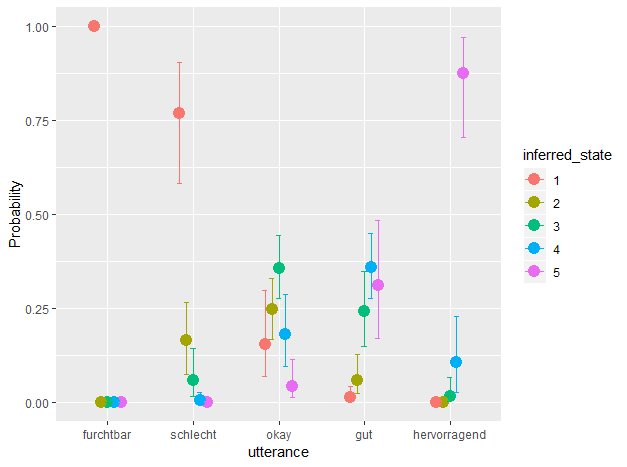
\includegraphics[width=\textwidth]{final_report/prob-inferred-state.png} 
\\
We test the following hypotheses: \\
\begin{enumerate}
\item Given the model and the data, is the inferred state credibly higher given a positive utterance for the honest condition than for the nice condition?
\item  Is the inferred state credibly higher for positive utterances for the nice condition than for the mean condition?
\item Is the inferred state credibly higher for negative utterances in the mean condition that in the honest condition?
\item Are the inferred states for negative utterances approximately same for honest and nice conditions?
\end{enumerate}
Given the model and the data, we could not verify any of the hypotheses ("Inferred states").
\\
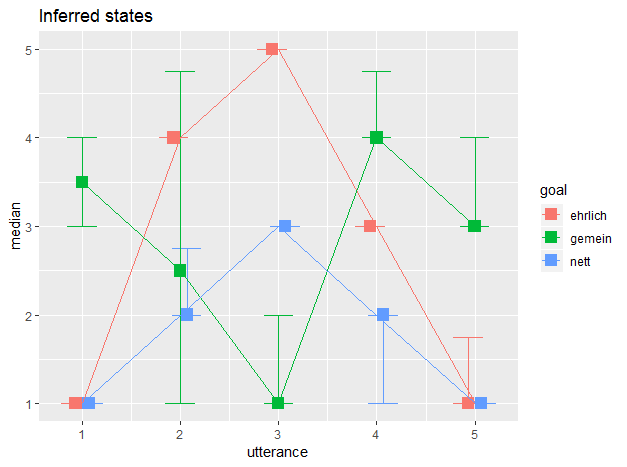
\includegraphics[width=15cm]{final_report/inferred-states.png} 
\\
We also fit a model including by-scenario and by-subject random effects. There is no significant difference between the fits.

\section{Discussion}
How do people interpret polite utterances? Does their interpretation depend on their language and culture? To our knowledge, there has been no direct cross-linguistic comparison made between listener's inferences upon polite utterances. With our replication study, we take a first step towards that. Furthermore, in terms of open science it is important to check prior findings for replicability. For more robust results, this study should be conducted with more participants in the future. The experimental design adapted here allows for specific context manipulation, however it produces counter-intuitive items like "Mary wants to be nice and says: "The cake was terrible"." An improvement of the paradigm should be worked out. 
\section{Conclusion}
Politeness is an omnipresent phenomenon in human language. The approach proposed by Brown and Levinson \cite{brown1987politeness} was adapted in this study and bears a great potential in terms of socially plausible language models. We could not verify that the states inferred by the listeners in German show the same ordinal relations depending on the communicative goal as in English, possibly due to the small amount of participants. Further investigation is necessary to draw more credible conclusions. 
\bibliography{references}
\bibliographystyle{ieeetr}



\end{document}
